\documentclass{article} % For LaTeX2e
\usepackage{final_project,times}
%\documentstyle[nips12submit_09,times,art10]{article} % For LaTeX 2.09
\usepackage{amsmath,amsthm,amsfonts,amssymb,amscd}
\usepackage{fullpage}
\usepackage{lastpage}
\usepackage{enumerate}
\usepackage{fancyhdr}
\usepackage{mathrsfs}
\usepackage{xcolor}
\usepackage[margin=2cm]{geometry}
\usepackage{fancyhdr} % Required for custom headers
\usepackage{lastpage} % Required to determine the last page for the footer
\usepackage{extramarks} % Required for headers and footers
\usepackage{graphicx} % Required to insert images
\usepackage{listings} % Required for insertion of code
\usepackage{framed}
\usepackage{courier}  % Required for the courier font
\usepackage{lipsum} % Used for inserting dummy 'Lorem ipsum' text into the template
\usepackage{float}
\usepackage{url}
\usepackage{bbm}
\usepackage{relsize}
\usepackage{amssymb}
\usepackage{fancyvrb}
\usepackage{amsmath}
\usepackage{mathrsfs}
\usepackage{algorithm}
\usepackage[noend]{algpseudocode}
\usepackage{amsmath}
\usepackage{listings}
\usepackage[none]{hyphenat}

\title{Optimizing Preseason Fantasy Football Rankings}

\author{
John O'Hollaren (jpo4) \\
Department of Electrical and Computer Engineering\\
}

\newcommand{\fix}{\marginpar{FIX}}
\newcommand{\new}{\marginpar{NEW}}

\nipsfinalcopy

\begin{document}


\maketitle

%#####################################################################################
%	Abstract
%#####################################################################################

\begin{abstract}
Fantasy football is a fast growing, multi-billion dollar industry centered around projecting which players will perform the best over the course of a season. Correctly predicting which players will play well greatly improves your team's year-long performance, whereas wasting a high pick on a low achiever can ruin your season. This paper focuses on an optimal strategy for predicting a list of the top 30 non-rookie NFL wide receivers for a season, using only data available prior to the start of the season.

\end{abstract}

%#####################################################################################
%	Introduction & Related Work
%#####################################################################################

\section{Introduction \& Related Work}

According to the Fantasy Sports Trade Association, over 10 percent of the US population spent 12 billion dollars playing fantasy football in 2012. Given such a large market, a slight statistical advantage could provide significant profits in fantasy football leagues. Specifically, a correct pre-season ranking of wide receivers (WRs) will allow owners to pick the best players to join their teams during the pre season fantasy football draft, setting them up for year-long success. However, ranking players is difficult. Preseason rankings from teams of experts at ESPN and Yahoo are correct for only a small minority of players. This paper compares several machine learning techniques for ranking WRs, including linear regression, feature reduction, K-Means clustering, mixture models, and PCA. A PCA regression technique which outperforms ESPN and Yahoo experts is presented. Throughout the paper, standard scoring is assumed: Fantasy Points = 6 $\cdot$ TDs + 0.1 $\cdot$ Yards.

While countless fantasy football websites exist, the major players are ESPN, Yahoo, the NFL, 4for4, and FantasyPros. None of these entities releases their methods publicly. Tim Mathews at the University of Southampton \cite{mathews} explored using Bayesian reinforcement learning for week-to-week team management during the season. Matt Bookman at Stanford used linear regression to predict week-to-week performances during the season with limited success only in certain weeks \cite{bookman}. The week-to-week prediction problem, however, is simplified through the use in-season data from each player, whereas in the pre-season, year-long ranking problem, predictions must be made for players who are 8 months removed from public games. Some attempts at machine learning approaches for the year-long ranking problem have been made \cite{kapania}, but did not outperform human experts. Other attempts use machine learning to outsmart other players in the same league \cite{becker}. 

\subsection{Data Summarization}

My dataset includes NFL statistics for over 700 players for every year from 2007 to 2012, however only a subset are used for prediction. There are 13 features in total. 6 are standard stats: yards, touchdowns, targets, catches, ESPN rank, and Yahoo rank. I then add a field for previous year points, and 6 more 'trend' features to represent trends over the years. For example: $\Delta 1yrYds = $  (Yards in year Y-1) - (Yards in year Y-2), $\Delta 2yrYds = $  (Yards in year Y-1) - (Yards in year Y-3). A total of 6 of these features are used, for both yards and touchdowns for 1, 2, and 3 years into the past, bringing the total to 13.

\subsection{Performance Criteria and Baseline}

Discounted cumulative gain (DCG) will be used to assess WR rankings. It rewards ranking good players highly and penalizes ranking bad players too high. A higher DCG is better:\\
$DCG = rel_1 + \sum\limits_{i=2}^{p} \frac{rel_i}{\log_2(i)}$, and the relevance weights are: $rel_i = \frac{1}{\text{actual end of year rank}}$ \\
Using DCG, the dataset can be analyzed by looking at the performance of ESPN, Yahoo, and simple regression across the years. Specifically note ESPN's 2012 DCG is 1.7991 and Yahoo's is 1.8100. These are the benchmarks for performance.

\begin{figure}[h]
\begin{centering}
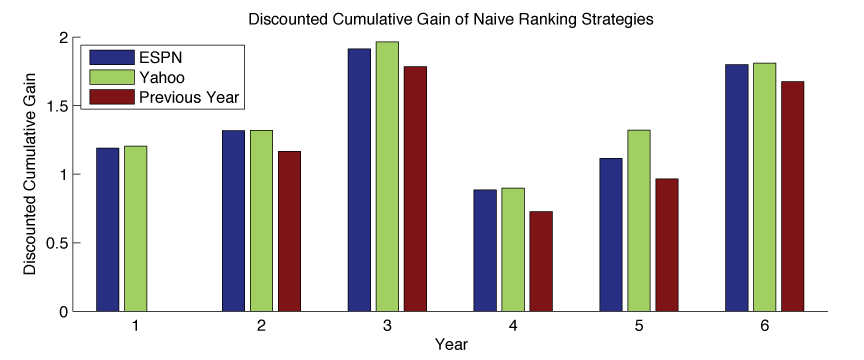
\includegraphics[width=5in]{media/dcg_naive.png}
\caption{DCG of ESPN/Yahoo preseason rankings by year, along with a na�ve method using the previous year�s final rankings as the next year�s preseason rankings. The 2012 results (1.7991 for ESPN, 1.8100 for Yahoo) will be used as a benchmark.}
\end{centering}
\end{figure}

\begin{figure}[h]
\begin{centering}
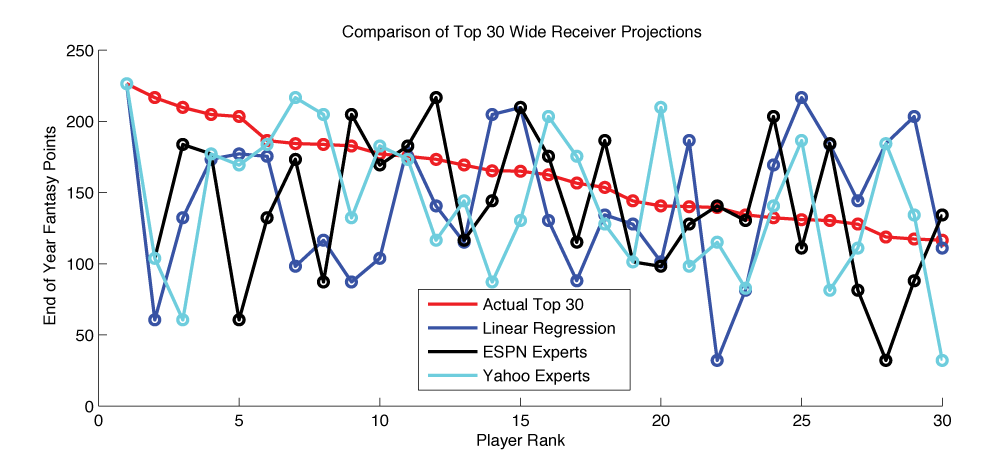
\includegraphics[width=5in]{media/top30_lin_reg_all_feat.png}
\caption{Preseason rankings versus actual points scored. Note how many of ESPN, Yahoo, and linear regression's preseason picks greatly underperform the actual best players in red. This graph shows how hard predicting rankings is.}
\end{centering}
\end{figure}

%#####################################################################################
%	Models and Methods
%#####################################################################################

\section{Models and Methods}

{\bf Linear Regression:} $\beta$ will be calculated using $X_{train}$ as all data up until 2010, and $Y_{train}$ as the 2011 end-of-season performances. $X_{test}$ will then be all data up until 2011, and the resulting $Y_{test} = \beta X_{test}$ will be the 2012 end-of-season performance which will be compared with the actual, ESPN, and Yahoo results using DCG. All features will be used for this 13-dimensional $\beta$. \\
$\beta = (X^T \cdot X)^{-1} \cdot X^T \cdot Y $ \\
$\beta = [ w_{Points}, w_{Yds}, w_{TDs}, w_{Targets}, w_{Catches}, w_{\Delta 1yrYds}, w_{\Delta 1yrTds}, w_{\Delta 2yrYds}, w_{\Delta 2yrTds}, w_{\Delta 3yrYds}, w_{\Delta 3yrTds}, w_{ESPN}, w_{Yahoo} ] $

{\bf Feature Reduction:} Feature reduction will be utilized to remove features that may not be necessary for prediction. This helps reduce computation overhead, allows the results to be easier to interpret because they are lower dimensional, and also can help reduce overfitting. Different subsets, $L$, of features will be experimented with for linear regression using $\beta_L = [ w_1 \dots w_L ]$. 

{\bf K-Means Mixture Model:} 2 and 3 dimensional K-Means will be used to separate players in different groupings, and linear regression will be run on each of the K mixtures individually. Each mixture, $1 \dots K$, will have it's own learned weights, $\beta_1 \dots \beta_K$. Both the features used for K-means and the number of features used for regression will be varied.

{\bf PCA Regression:} PCA will be used to estimate the regression coefficients. Different numbers of principle components will be experimented with. PCA on X gives a principle component score, $\Omega_{n \times p}$ = a representation of X in the principle component space, and also the principle component loadings in each column of $\Lambda_{p \times p}$. $\beta$ is initially estimated as before, but by replacing X with $\Omega$ and mean centering $Y$ to give: $\beta = (\Omega^T \cdot \Omega)^{-1} \cdot \Omega^T \cdot (Y - \mu_Y) $. Then to make the results easier to interpret, $\beta$ is transformed to regression coefficients for uncentered variables by adding a mean term and adding a column of 1's to X during prediction: $\beta = [ \mu_Y - \mu_X \cdot \Lambda \cdot \beta | \Lambda \cdot \beta ]$, $Y = [1's | X ] \cdot \beta$.

%#####################################################################################
%	Results
%#####################################################################################

\section{Results}

Using linear regression, $\beta$ is calculated and then used to predict point totals for each player at the end of the next year. The top 30 players are then ranked by their point totals, and the ranking is scored using DCG. Note that as we use more training data, the RMSE of the point predictions reduces, which in turn leads to the DCG increasing as shown in Figure \ref{fig:learn}.

%\begin{figure}[h]
%\begin{centering}
%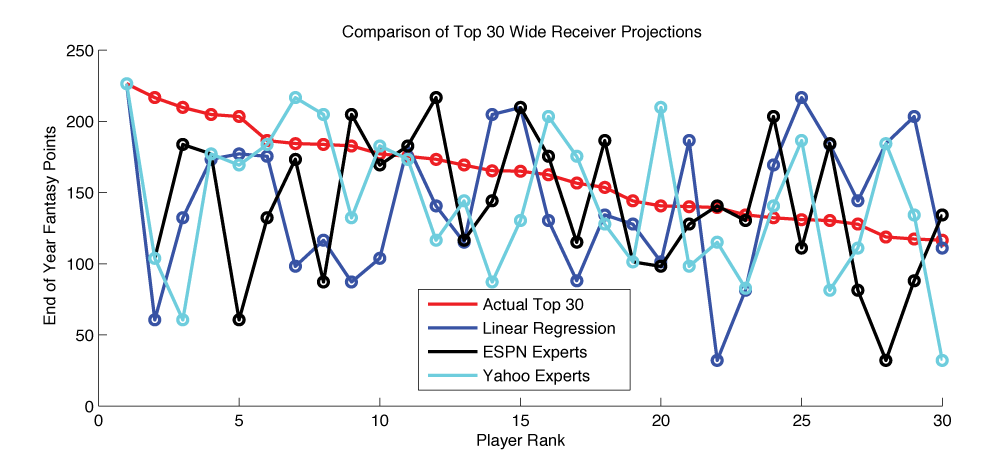
\includegraphics[width=5in]{media/top30_lin_reg_all_feat.png}
%\caption{: DCG of ESPN / Yahoo preseason rankings over the years, along with a na�ve method of using the previous year�s final rankings as the next year�s preseason rankings.}
%\end{centering}
%\end{figure}

\begin{figure}[h]
\begin{centering}
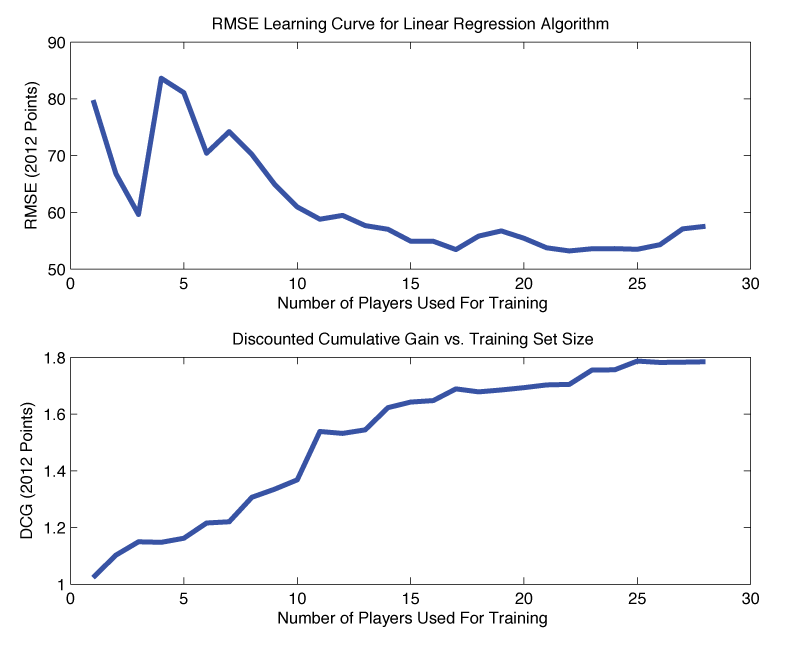
\includegraphics[width=4in]{media/lin_reg_learning_curve.png}
\caption{Graph of RMSE and DCG as the training set size increases. Results improve with larger training sets.}
\label{fig:learn}
\end{centering}
\end{figure}

The linear regression results can be improved by picking out specific features to perform regression on. Multiple combinations of features were experimented with. The best results were shown with less than the full 13 features. Specifically, 2, 3, and 7 feature regression worked well on the features as shown in Table \ref{tab:red}.

\begin{table}[ht] 
\centering % used for centering table 
\begin{tabular}{c c c} % centered columns (4 columns) 
\hline\hline %inserts double horizontal lines 
\# Features & Features & DCG \\% inserts table 
%heading 
\hline % inserts single horizontal line 
13 & Points, Yds, TDs, Targets, Catches, $\Delta 1yds$, $\Delta 1yds$, $\Delta 2yds$, $\Delta 2tds$, $\Delta 3yds$, $\Delta 3tds$, ESPN, Yahoo & 1.7179 \\  
7 & Points, Yds, TDs, Targets, Catches, $\Delta 1yds$, $\Delta 1yds$, ESPN, Yahoo & 1.7722 \\  
6 & Points, Yds, TDs, Targets, Catches, $\Delta 1yds$, $\Delta 1yds$, ESPN & 1.7621 \\  
3 & Points, Yds, TDs & 1.7806 \\  
2 & Points, TDs & 1.7896 \\  
2 & Points, Yds & 1.7863 \\ 
\hline %inserts single line 
\end{tabular} 
\caption{Results of feature reduction showing improved results in lower dimensional spaces.}
\label{tab:red}
\end{table} 

Feature reduction greatly improves the results! However, performance is still short of experts at ESPN and Yahoo. Now the method takes advantage of the fact that there are many types of receivers in the NFL, including those who play in the slot and catch lots of short passes, those who play out wide and catch very few longer passes, and all-stars who do it all. This insight prompts clustering receivers by type period to prediction, which is done using K-Means as shown in Figure \ref{fig:means}. 

\begin{figure}[h]
\begin{centering}
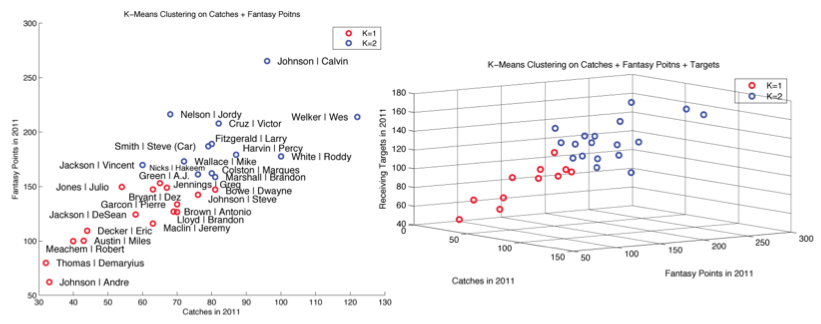
\includegraphics[width=7in]{media/kmeans.png}
\caption{Results of k-means clustering in 2 and 3 dimensions.}
\label{fig:means}
\end{centering}
\end{figure}

After grouping players using K-Means, each group is predicted individually. Feature reduction is employed by using both 2 and 6 features. The results of each mixture's predictions are then combined to produce a single top 30 WR list for 2012, which is then scored using DCG as shown in Table \ref{tab:km}. A DCG of 1.8063 is obtained, which beats ESPN, but not Yahoo.

\begin{table}[ht] 
\centering % used for centering table 
\begin{tabular}{c c c c} % centered columns (4 columns) 
\hline\hline %inserts double horizontal lines 
\# Mixtures & K-Means Features & DCG (6 Features) & DCG (2 Features) \\% inserts table 
%heading 
\hline % inserts single horizontal line 
2 & Catches, Fantasy Points & 1.7601 & 1.8063 \\
2 & Fantasy Points & 1.7601 & 1.7925 \\
3 & Fantasy Points & 1.3621 & 1.7880 \\
2 & Targets & 1.2053 & 1.7877 \\
2 & Catches, Fantasy Points, Targets & 1.1887 & 1.7863 \\
2 & Catches & 1.1811 & 1.7814 \\
2 & Touchdowns & 1.1107 & 1.7747 \\
2 & Yards & 1.0857 & 1.4428 \\
\hline %inserts single line 
\end{tabular} 
\caption{K-Means mixture model results through several types of runs.}
\label{tab:km}
\end{table} 

The results of PCA and PCA Regression in Figure \ref{fig:pca} show that the majority of the variance in our data is explained by the first 4 principle components. Using PCA regression with 10 principle components, we are able to out-perform the experts at both Yahoo and ESPN by producing a DCG of 1.8132.

\begin{figure}[h]
\begin{centering}
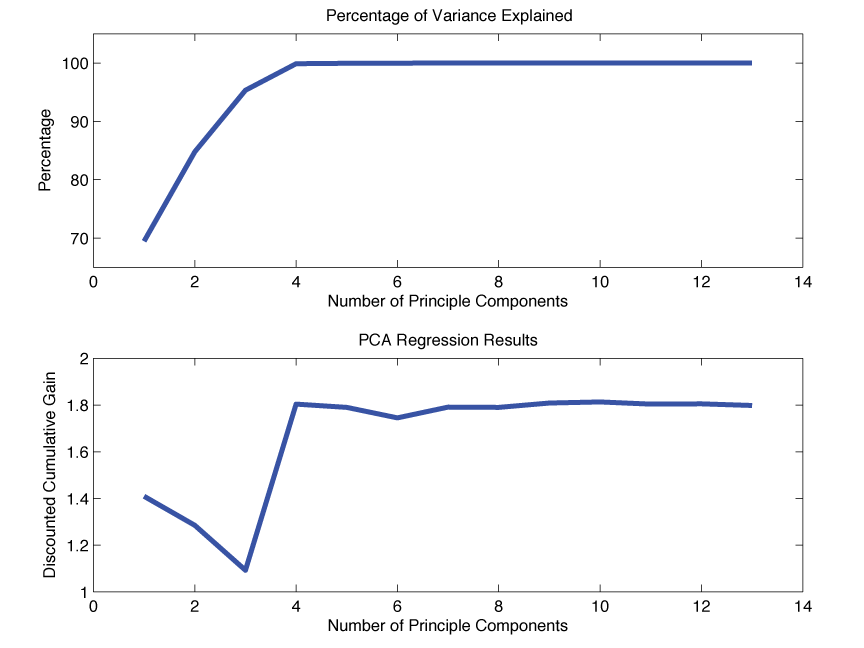
\includegraphics[width=4in]{media/pca.png}
\caption{PCA and PCA regression run with varying numbers of principle components. Note how the DCG goes up as enough principle components are chosen to explain the majority of the variance.}
\label{fig:pca}
\end{centering}
\end{figure}

%#####################################################################################
%	Conclusions
%#####################################################################################

\section{Conclusions}

Several machine learning approaches to ranking NFL receivers are shown. The best results come from PCA regression with 10 principle components. This method outperforms the experts at ESPN and Yahoo for the 2012 season. Future work could include examining expanding this to predict which players will have the best careers, predicting 2 or 3 years in advance, and refining the model by incorporating more data from previous years.

%#####################################################################################
%	Bibliography
%#####################################################################################

\newpage

\section{Bibliography}

\begin{thebibliography}{1}

\bibitem{mathews} Mathews, Tim, et. al. �Competing with Humans at Fantasy Football: Team Formation in Large Partially-Observable Domain.� Association for the Advancement of Artificial Intelligence, 2012.

\bibitem{bookman} Bookman, Matt. "Predicting Fantasy Football - Truth in Data." Stanford CS 229 Final Project. December 14, 2012.

\bibitem{kapania} Kapania, Nitin. "Predicting Fantasy Football Performance with Machine Learning Techniques." Stanford CS 229 Final Project. December 14, 2012.

\bibitem{becker} Becker, Adrian, et. al. "An Analytical Approach for Fantasy Football Draft and Lineup Management." MIT ORC Technical Report. November 2010.

\end{thebibliography}
  
\end{document}


